\usetikzlibrary{calc}
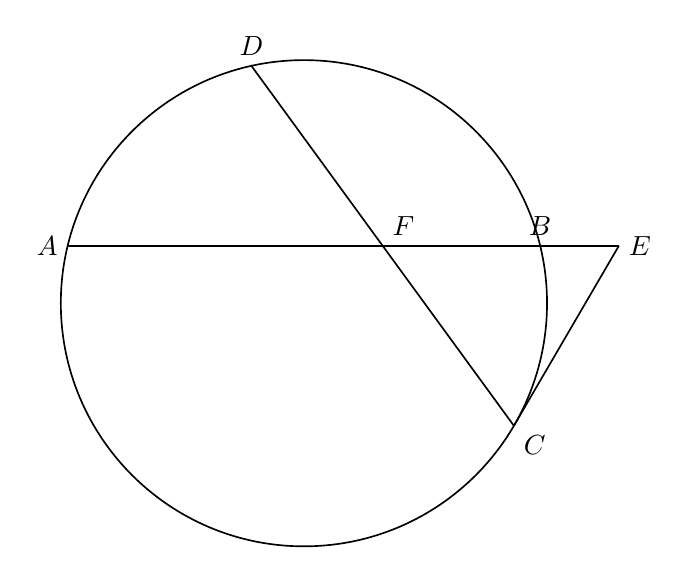
\begin{tikzpicture}[x=1cm,y=1cm,line width=.6pt,font=\normalsize]
\coordinate (A) at (-4.0,0.0);
\coordinate (F) at (0.0,0.0);
\coordinate (B) at (2.0,0.0);
\coordinate (E) at (3.0,0.0);
\coordinate (D) at (-1.66667,2.28522);
\coordinate (C) at (1.66667,-2.28522);
\coordinate (O) at (-1.0,-0.72932);
\draw (O) circle[radius=3.08738cm];
\draw (A)--(E);
\draw (D)--(C);
\draw (C)--(E);
\node[left] at (A) {$A$};
\node[above] at (D) {$D$};
\node[above right] at (F) {$F$};
\node[above] at (B) {$B$};
\node[right] at (E) {$E$};
\node[below right] at (C) {$C$};
\end{tikzpicture}
